\documentclass[border=0.2cm]{standalone}

\usepackage[utf8]{inputenc}
\usepackage[T1]{fontenc}
\usepackage{amsmath}
\usepackage{helvet}
\usepackage{tikz}

\usetikzlibrary{arrows.meta}
\usetikzlibrary{positioning, calc, fit}
\usetikzlibrary{decorations.markings}
\usetikzlibrary{shapes.geometric, shapes.arrows}

\renewcommand\familydefault\sfdefault


\begin{document}

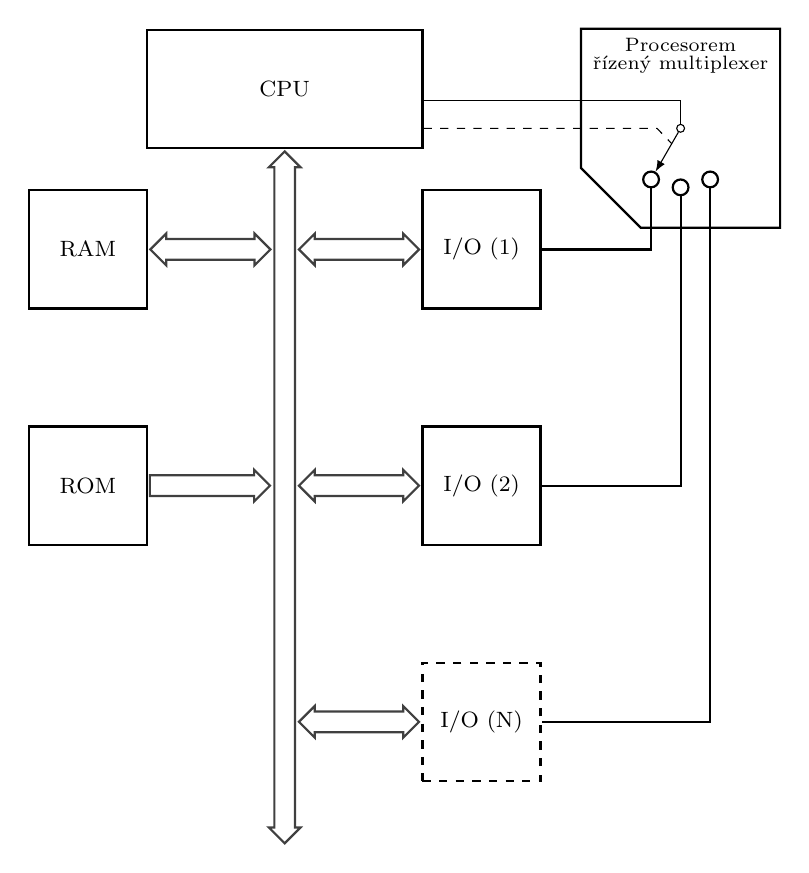
\begin{tikzpicture}[
    square/.style={regular polygon,regular polygon sides=4},
    d arrow/.style={gray!50!black, thick, double arrow, draw, minimum width = 8pt, double arrow head extend=2pt, anchor=tip 2},
    s arrow/.style={gray!50!black,thick, single arrow, draw, minimum width = 8pt, single arrow head extend=2pt},
    block/.style={thick, draw, font=\footnotesize},
    square/.style={block, minimum size=1.5cm},
    pin/.style={font=\scriptsize}
]
    \draw  node[square] (ram) {$ \text{RAM} $} ;
    \draw  (ram) ++(0, -3) node[square] (rom) {$ \text{ROM} $} ;

    \draw (ram) ++(5, 0) coordinate (io_origin);
    \foreach \e [count=\i from 0] in {1, 2} {
        \draw  (io_origin) ++(0, -3*\i) node[square] (io\i) {$ \text{I/O (\e)} $};
    }

    \draw  (io1) ++(0, -3) node[square, dashed] (ioN) {$ \text{I/O (N)} $};
    
    \draw ($(ram.north)!.5!(io0.north)$) ++(0, .5) node [d arrow, minimum height=250, rotate=-90] (bus) {};

    \draw ($(bus.tip 2) + (0, .01)$)  node[block, minimum width=3.5cm, minimum height=1.5cm, anchor=south] (cpu) {$ \text{CPU} $};

    \draw (cpu.north east) ++(2, 0) node [anchor=north west, thick, minimum width=2.5cm, minimum height=2.5cm] (mux) {};
    \node[pin, below, align=center] at (mux.north){Procesorem\\[-0.2em] řízený multiplexer};

    \draw [thick] (mux.north west) -- (mux.north east) -- (mux.south east) -- ($ (mux.south east)!.7!(mux.south west)$) -- ($ (mux.north west)!.7!(mux.south west)$) -- cycle;

    \draw (mux.base) node[draw, circle, minimum size=.1cm, inner sep=0pt] (pivot) {};
    
    \foreach \p in {0, ..., 2} {
        \draw (pivot) ++(-\the\numexpr\p*30+60\relax:.75cm) node[thick, draw, circle, minimum size=.2cm, inner sep=0pt] (i\p) {};
    }
    \foreach \io/\i in {0/2, 1/1, N/0} {
        \draw[thick] (i\i) |- (io\io);
    }

    % Side-to-Center arrows:
    \draw let \p1=(ram.east), \p2=($ (ram.east)!.5!(io0.west) -(6pt, 0) $), \n1={veclen(\y2-\y1,\x2-\x1)} in ($ (ram.east) + (0.01, 0)$) node [d arrow, minimum height=\n1] {};
    \draw let \p1=(rom.east), \p2=($ (rom.east)!.5!(io1.west) -(6pt, 0) $), \n1={veclen(\y2-\y1,\x2-\x1)} in ($(rom.east) + (0.01, 0)$) node [s arrow, minimum height=\n1, anchor=tail] {};
    \draw let \p1=(io0.west), \p2=($ (ram.east)!.5!(io0.west) +(6pt, 0) $), \n1={veclen(\y2-\y1,\x2-\x1)} in ($(io0.west) + (-0.01, 0)$) node [d arrow, minimum height=\n1, rotate=180] {};
    \draw let \p1=(io1.west), \p2=($ (rom.east)!.5!(io1.west) +(6pt, 0) $), \n1={veclen(\y2-\y1,\x2-\x1)} in ($(io1.west) + (-0.01, 0)$) node [d arrow, minimum height=\n1, rotate=180] {};   
    \draw let \p1=(ioN.west), \p2=($ (rom.east|-ioN.west)!.5!(ioN.west) +(6pt, 0) $), \n1={veclen(\y2-\y1,\x2-\x1)} in ($(ioN.west) + (-0.01, 0)$) node [d arrow, minimum height=\n1, rotate=180] {};

    \draw[-latex] (pivot) -- (i2);
    \draw(pivot) -- ++(0, .35) to (cpu.east|-\tikztostart);
    \draw[dashed] (cpu.east|-pivot) -- ($ (pivot) - (0.3,0) $) -- ($ (pivot)!.3!(i2) $);

\end{tikzpicture}
\end{document}
